% Updated in May 2014 by Hideo Saito
% Updated in March 2012 by Yasuyuki Matsushita
% Updated in April 2002 by Antje Endemann, ...., and in March 2010 by Reinhard Klette
% Based on CVPR 07 and LNCS style, with modifications by DAF, AZ and elle 2008, AA 2010, ACCV 2010

\documentclass[runningheads]{llncs}
\usepackage{graphicx}
\usepackage{amsmath,amssymb} % define this before the line numbering.
\usepackage{ruler}
\usepackage{color}

\usepackage{epstopdf}
\usepackage{times}
\usepackage{epsfig}
\usepackage{graphicx}
\usepackage{url}
\usepackage{bm}

%===========================================================
\begin{document}
\pagestyle{headings}
\mainmatter


\def\ACCV14SubNumber{215}  % Insert your submission number here

%===========================================================
\title{Clouds in The Cloud\\
Supplementary Material}
\titlerunning{ACCV-14 submission ID \ACCV14SubNumber - Supplementary Material}
\authorrunning{ACCV-14 submission ID \ACCV14SubNumber - Supplementary Material}

\author{Anonymous ACCV 2014 submission}
\institute{Paper ID \ACCV14SubNumber}

\maketitle

%===========================================================
\section{Simulations}

We used simulated data to test the camera network concept
quantitatively and to scale it to large number of cameras. In this
section we detail the simulation setup and results.

% -------------------------------------------------------------------------
\subsection{Setup}

To synthesize cloud images we SHDOM~\cite{Evans1998}, a Radiative
Transfer solver based on the discrete ordinate spherical-harmonic
method. As input to the SHDOM we used a Liquid Water Content (LWC)
field created by the UCLA Large-Eddy Simulation (LES)
code~\cite{(stevens_evaluation_2005)}.  The LWC field spans
$8000\times 8000 \time 1500{\rm m}^3$ grid and represents sparse
Cumulus clouds heights of $500{\rm m}$ to $1500{\rm
  m}^2$. Fig.~\ref{fig:simulation_imgs2}(a) shows a $2500 \times
2500{\rm m}$ subset of the grid.  The solar zenith angle was set to
$\frac{\pi}{4}$.  We synthesized images taken from 100 cameras placed
on an evenly spaced grid over a $2500\times 2500{\rm m}^2$ domain.  We
simulated a static Sun-blocker consistent with Copenhagen (unrelated
to the anonymous authors) Latitude.

\begin{figure}
  \begin{center}
    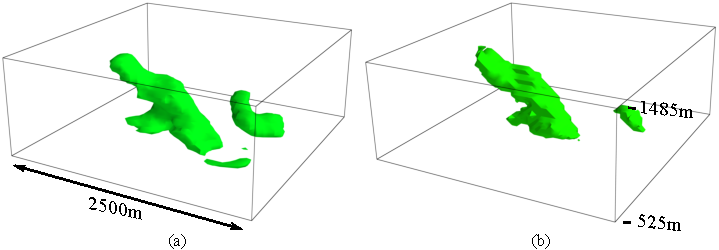
\includegraphics{figures/clouds3d_SHDOM}
    \caption{Cloud reconstruction results: (a) The water liquid
      distribution used as input to the SHDOM simulation. (b)
      Reconstructed clouds.}
    \label{fig:simulation_imgs2}
  \end{center}
\end{figure}

% -------------------------------------------------------------------------
\subsection{Results}

Figs.~\ref{fig:simulation_imgs1}(a,b) show images from two out of 100
synthesized cameras. Figs.~\ref{fig:simulation_imgs1}(c,d) show the
same images with the simulated Sun-blocker applied.
Fig.~\ref{fig:simulation_imgs2}(b) shows the result of the
reconstruction algorithm described in our article. We reconstructed
only the cloud distribution in the atmosphere above cameras (marked by
Red triangle in Figs.~\ref{fig:simulation_imgs1}(a,b)).
\begin{figure}
  \begin{center}
    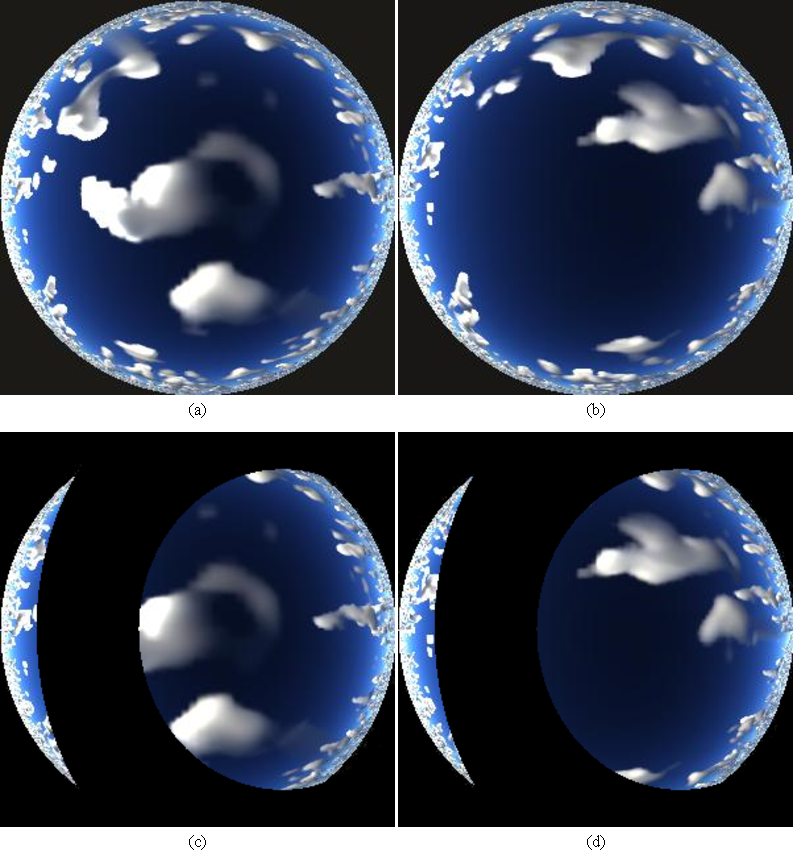
\includegraphics{figures/simulation_imgs}
    \caption{Images synthesised using SHDOM and used in the
      reconstruction algorithm: (a,b) Two images (out of 100) of the
      same scene from different cameras. Red rectangle marks the
      Region Of Interest of the reconstruction algorithm. (c,d) The
      same images with the simulated sun-blocker applied.}
    \label{fig:simulation_imgs1}
  \end{center}
\end{figure}

To test the performance of the camera network as function of its size
we used random subsets of the network, where the whole images are
taken either with or without a sun blocker. The different network
subsets were compared based on their cloud classification score.  In
the LES, a voxel is occupied by cloud if its water-mass parameter is
not null. In the recovery, voxel $k$ is classified as cloud if
$T_k>0.01$.  We measured the classification error rate, across all
voxels.  The results are plotted in Fig.~\ref{fig:simulations}.  As
expected of space carving, results improve fast from 2 to 10
cameras. Even when a sun blocker is applied, the algorithm is able to
reconstruct the cloud formation. Then, as expected, more cameras are
needed in order to compensate for the limited view of each camera. In
our setup the cameras observe the clouds only from below. This is the
classical limited angle problem known from visual hull and tomography
algorithms. Therefore the reconstruction error does not converge to
zero.

\begin{figure}
  \begin{center}
    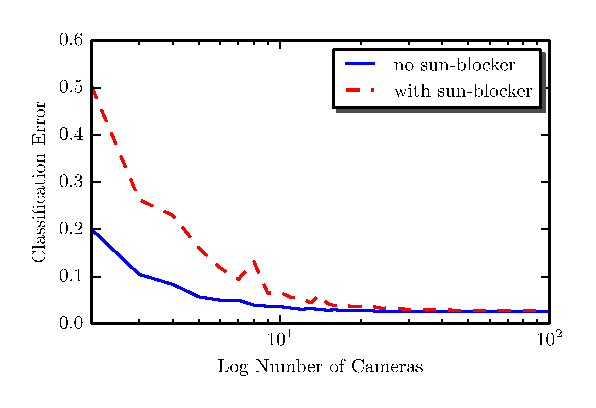
\includegraphics{figures/simulations.eps}
    \caption{Classification error rate as a function of the number of
      cameras. [Solid Blue] Without sun blocker. [Dashed Red] With sun
      blocker.  Fluctuations are within the random sampling standard
      deviation.}
    \label{fig:simulation}
  \end{center}
\end{figure}


% ===========================================================
\section{SIFT}

%%%%%%%%%%%%%%%%%%%%%%%%%%%%%%%%%%%%%%%%%%%%%%%%%%%%%%%%%%%%%%
\subsection*{Spatial similarity score}
\label{sec:appearancecore}

During our experiments, we had found that simple color consistency was not enough when tackling difficult cloud structures such as high-altitude ciruss due to spatial ambiguity and very low baseline between the cameras. In such cases spatial information would be a natural way of incorporating a multi-view stereo approach into our space-carving scheme.
Dense SIFT~\cite{DenseSift2011} has been recently proven to be an efficient feature for non-rigid matching between pairs of images.
In a similar manner, dense SIFT can be incorporated in our multi-view probablistic space-carving scheme to represent the structural appearance of a projected voxel. SIFT descriptors also give us the benefit of robustness under scale and view-angle variations.
Voxel $k$ projects to a subset of the rays $\rho_k\subset{\cal R}$,
that reach $\nu_k$ viewpoints.
For each of the rays $r\in\rho_k$ at time $t$, we sample the 3 RGB values and compute the 128-bin SIFT descriptor for the 8x8 patch surrounding the ray.
The resulting feature vector ${\bf v}(r,t)$ is a weighted concatenation of the RGB values and the 128-bin SIFT vector.

Spatial similarity score in defined as a simple sum of variences in the different components of the feature vectors:
\begin{equation}
 P_k= \exp\left(
         -\Sigma_q\{VAR[{\cal V}_q(k,t)]\}/\sigma^2
         \right)
  \;,
 \label{eq:Dist}
\end{equation}
where $q=\{1..131\}$ and $\sigma^2$ is a global scale parameter.




%===========================================================
\bibliographystyle{splncs}
\bibliography{cloudsbib}

%this would normally be the end of your paper, but you may also have an appendix
%within the given limit of number of pages
\end{document}
